
\documentclass[12pt]{exam}
\usepackage{amsthm}
\usepackage{libertine}
%\usepackage[utf8]{inputenc}
\usepackage[margin=1in]{geometry}
\usepackage{amsmath,amssymb}
\usepackage{multicol}
\usepackage[shortlabels]{enumitem}
\usepackage{siunitx}
\usepackage{cancel}
\usepackage{graphicx}
\graphicspath{{./}}
\usepackage{pgfplots}
\usepackage{hyperref}
\usepackage{listings}
\usepackage{tikz}
\usepackage{minted}
\def\code#1{\texttt{#1}}
\usepackage{amssymb}
\usepackage{xcolor}
% for plotting
\usepackage{pgfplots}
\pgfplotsset{compat=1.16}
\usepackage{tikz}
\usetikzlibrary{arrows.meta}

\newcommand{\quotebox}[1]
{
  \begin{center}
    \fcolorbox{white}{blue!15!gray!15}{
      \begin{minipage}{0.7\linewidth}\vspace{10pt}
        \center
        \begin{minipage}{0.8\linewidth}{\space\Huge``}{\setlength{\parindent}{1.5em}#1}{\hspace{1.5em}\break\null\Huge\hfill''}
        \end{minipage}
        \smallbreak
      \end{minipage}
    }
\end{center}
}


% for plotting half circle
% call it with \MyHalfCircle{<size>}{<x coord>}{<y coord>} in tikz pictur
\newcommand{\MyHalfCircle}[3][0.4ex]{%
    % #1 = size
    % #2 = x coordinate
    % #3 = y coordinate
  \begin{scope}
   \draw (axis cs:#2,#3) circle (#1);
   \clip (axis cs:#2,#3) circle (#1);
   \fill[red, opacity=0.75] (axis cs:#2,#1) rectangle (axis cs:-#1,-#1);
  \end{scope}
}




%\DeclareUnicodeCharacter{2212}{-}


\let\oldemptyset\emptyset
\let\emptyset\varnothing

\hypersetup{
    colorlinks=true,
    linkcolor=blue,
    filecolor=magenta,      
    urlcolor=cyan,
    pdftitle={Overleaf Example},
    pdfpagemode=FullScreen,
    }
    
\urlstyle{same}

\pgfplotsset{width=10cm,compat=1.9}
\usepgfplotslibrary{external}
\tikzexternalize

\newcommand{\class}{Math 415} % This is the name of the course 
\newcommand{\examnum}{Homework-3} % This is the name of the assignment
\newcommand{\examdate}{Sep 27} % This is the due date
\newcommand{\timelimit}{}

\newcommand{\BO}{\mathcal{O}}




\begin{document}
\pagestyle{plain}
\thispagestyle{empty}

\noindent
\begin{tabular*}{\textwidth}{l @{\extracolsep{\fill}} r @{\extracolsep{6pt}} l}
\textbf{\class} & \textbf{Name:} & \textit{Zhenzhao Tu}\\ %Your name here instead, obviously 
\textbf{\examnum} &&\\
\textbf{\examdate} &&\\
\end{tabular*}\\
\rule[2ex]{\textwidth}{2pt}
% --


\section*{Problem 1}
For ODE $x'=1+rx+x^2$, we will find the Bifurcation diagram.
\begin{enumerate}[(a)]
	\item When $r>2$, we can sketch the vector field as below:
	
		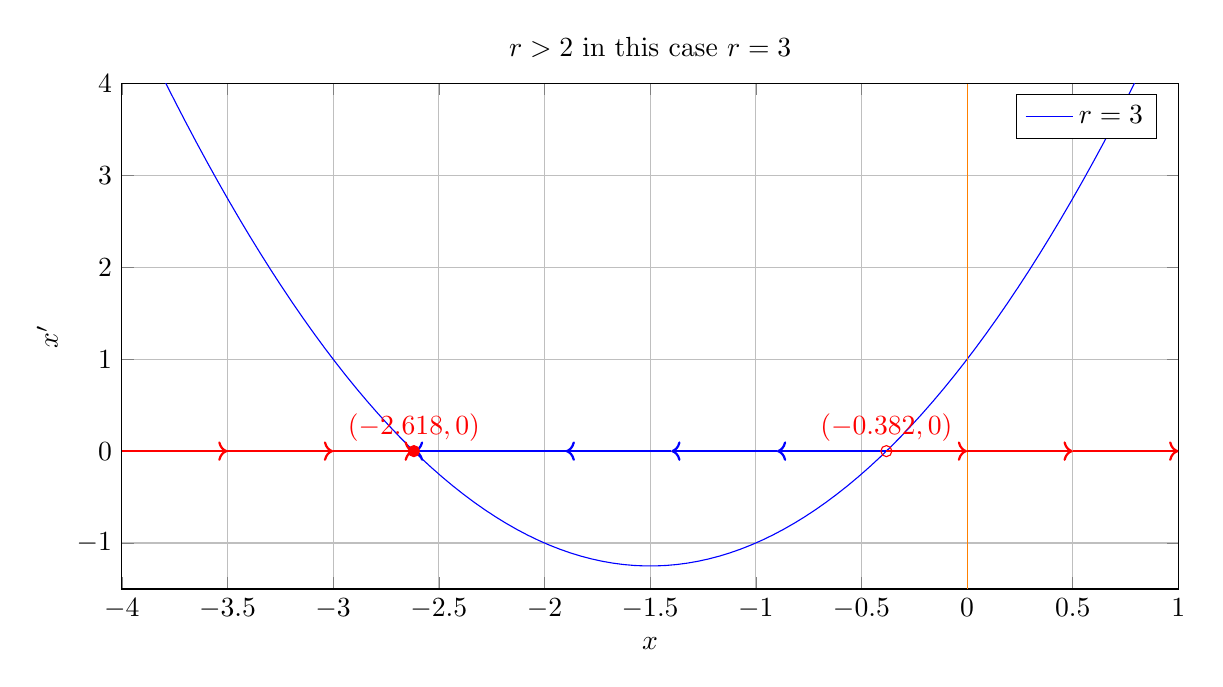
\begin{tikzpicture}
		\begin{axis}[
			title = {$r>2$ in this case $r=3$},
			xlabel = {$x$},
			ylabel = {$x'$},
			xmin = -4, xmax = 1,
			ymin = -1.5, ymax = 4,
			grid = major,
			width=15cm,
			height=8cm,
			]

			% when r=3
			\addplot[blue, domain=-4:1, samples=100] {1+3*x+x^2};
			% add horizontal line x=0
			\addplot[orange, domain=-4:1, samples=100] {0};
			% add vertical line y=0
			\addplot[orange, domain=-4:1, samples=100] coordinates {(0,-1.5) (0,4)};

			% add hollow point at (-0.382,0)
			\addplot[only marks, mark=o, mark size=2pt, color=red] coordinates {(-0.382,0)} node[above]{$(-0.382,0)$};
			% add point at (-2.618,0) with label
			\addplot[only marks, mark=*, mark size=2pt, color=red] coordinates {(-2.618,0)} node[above]{$(-2.618,0)$};

			% draw vector form (-4,0) to (-3.5,0) and change the arrow to thick
			\addplot[->, thick, color=red] coordinates {(-4,0) (-3.5,0)};
			% draw vector form (-3.5,0) to (-3,0) and change the arrow to thick
			\addplot[->, thick, color=red] coordinates {(-3.5,0) (-3,0)};
			% draw vector form (-3,0) to (-2.618,0) and change the arrow to thick
			\addplot[->, thick, color=red] coordinates {(-3,0) (-2.618,0)};
			% draw vector form (-0.382,0) to (0,0) and change the arrow to thick
			\addplot[->, thick, color=red] coordinates {(-0.382,0) (0,0)};
			% draw vector form (0,0) to (0.5,0) and change the arrow to thick
			\addplot[->, thick, color=red] coordinates {(0,0) (0.5,0)};
			% draw vector form (0.5,0) to (1,0) and change the arrow to thick
			\addplot[->, thick, color=red] coordinates {(0.5,0) (1,0)};

			% draw vector form (-0.382,0) to (-0.9,0) and change the arrow to thick
			\addplot[->, thick, color=blue] coordinates {(-0.382,0) (-0.9,0)};
			% draw vector form (-0.9,0) to (-1.4,0) and change the arrow to thick
			\addplot[->, thick, color=blue] coordinates {(-0.9,0) (-1.4,0)};
			% draw vector form (-1.4,0) to (-1.9,0) and change the arrow to thick
			\addplot[->, thick, color=blue] coordinates {(-1.4,0) (-1.9,0)};
			% draw vector form (-1.9,0) to (-2.618,0) and change the arrow to thick
			\addplot[->, thick, color=blue] coordinates {(-1.9,0) (-2.618,0)};

			\legend{$r=3$}
		\end{axis}
		\end{tikzpicture}
	
	\item When $r=2$, we can sketch the vector field as below:
	
		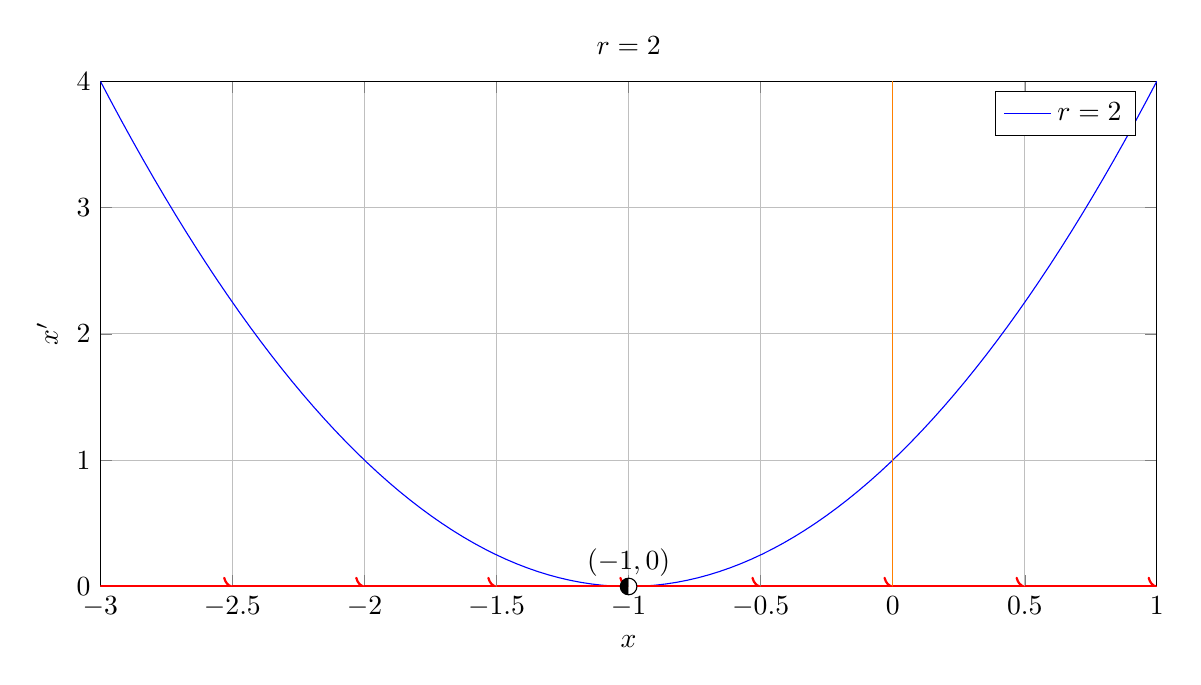
\begin{tikzpicture}
		\begin{axis}[
			title = {$r=2$},
			xlabel = {$x$},
			ylabel = {$x'$},
			xmin = -3, xmax = 1,
			ymin = 0, ymax = 4,
			grid = major,
			width=15cm,
			height=8cm,
			]

			% when r=2
			\addplot[blue, domain=-3:1, samples=100] {1+2*x+x^2};
			% add horizontal line x=0
			\addplot[orange, domain=-4:1, samples=100] {0};
			% add vertical line y=0
			\addplot[orange, domain=-4:1, samples=100] coordinates {(0,-1.5) (0,4)};

			% add half circle at (-1,0)
			\addplot[mark=halfcircle*, mark options={rotate=90}, mark size=3pt] coordinates {(-1, 0)} node[above]{$(-1,0)$};

			% draw vector form (-3,0) to (-2.5,0) and change the arrow to thick
			\addplot[->, thick, color=red] coordinates {(-3,0) (-2.5,0)};
			% draw vector form (-2.5,0) to (-2,0) and change the arrow to thick
			\addplot[->, thick, color=red] coordinates {(-2.5,0) (-2,0)};
			% draw vector form (-2,0) to (-1.5,0) and change the arrow to thick
			\addplot[->, thick, color=red] coordinates {(-2,0) (-1.5,0)};
			% draw vector form (-1.5,0) to (-1,0) and change the arrow to thick
			\addplot[->, thick, color=red] coordinates {(-1.5,0) (-1,0)};
			% draw vector form (-1,0) to (-0.5,0) and change the arrow to thick
			\addplot[->, thick, color=red] coordinates {(-1,0) (-0.5,0)};
			% draw vector form (-0.5,0) to (0,0) and change the arrow to thick
			\addplot[->, thick, color=red] coordinates {(-0.5,0) (0,0)};
			% draw vector form (0,0) to (0.5,0) and change the arrow to thick
			\addplot[->, thick, color=red] coordinates {(0,0) (0.5,0)};
			% draw vector form (0.5,0) to (1,0) and change the arrow to thick
			\addplot[->, thick, color=red] coordinates {(0.5,0) (1,0)};

			\legend{$r=2$}
		\end{axis}	
		\end{tikzpicture}

	\item When $-2<r<2$, we can sketch the vector field as below:

		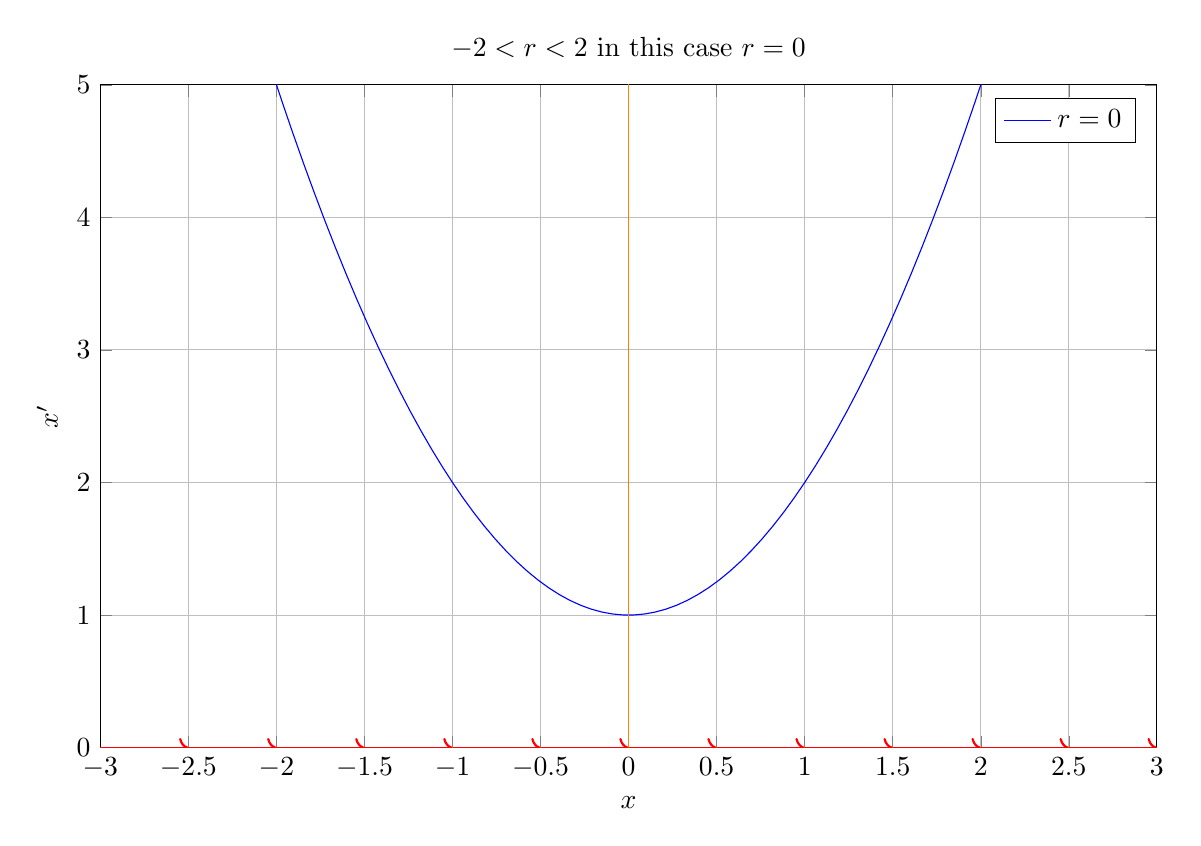
\begin{tikzpicture}
		\begin{axis}[
			title = {$-2<r<2$ in this case $r=0$},
			xlabel = {$x$},
			ylabel = {$x'$},
			xmin = -3, xmax = 3,
			ymin = 0, ymax = 5,
			grid = major,
			width=15cm,
			height=10cm,
			]

			% when r=0
			\addplot[blue, domain=-3:3, samples=100] {1+x^2};
			% add horizontal line x=0
			\addplot[orange, domain=-3:3, samples=100] {0};
			% add vertical line y=0
			\addplot[orange, domain=-3:3, samples=100] coordinates {(0,0) (0,6)};

			
			% draw vector form (-3,0) to (-2.5,0) and change the arrow to thick
			\addplot[->, thick, color=red] coordinates {(-3,0) (-2.5,0)};
			% draw vector form (-2.5,0) to (-2,0) and change the arrow to thick
			\addplot[->, thick, color=red] coordinates {(-2.5,0) (-2,0)};
			% draw vector form (-2,0) to (-1.5,0) and change the arrow to thick
			\addplot[->, thick, color=red] coordinates {(-2,0) (-1.5,0)};
			% draw vector form (-1.5,0) to (-1,0) and change the arrow to thick
			\addplot[->, thick, color=red] coordinates {(-1.5,0) (-1,0)};
			% draw vector form (-1,0) to (-0.5,0) and change the arrow to thick
			\addplot[->, thick, color=red] coordinates {(-1,0) (-0.5,0)};
			% draw vector form (-0.5,0) to (0,0) and change the arrow to thick
			\addplot[->, thick, color=red] coordinates {(-0.5,0) (0,0)};
			% draw vector form (0,0) to (0.5,0) and change the arrow to thick
			\addplot[->, thick, color=red] coordinates {(0,0) (0.5,0)};
			% draw vector form (0.5,0) to (1,0) and change the arrow to thick
			\addplot[->, thick, color=red] coordinates {(0.5,0) (1,0)};
			% draw vector form (1,0) to (1.5,0) and change the arrow to thick
			\addplot[->, thick, color=red] coordinates {(1,0) (1.5,0)};
			% draw vector form (1.5,0) to (2,0) and change the arrow to thick
			\addplot[->, thick, color=red] coordinates {(1.5,0) (2,0)};
			% draw vector form (2,0) to (2.5,0) and change the arrow to thick
			\addplot[->, thick, color=red] coordinates {(2,0) (2.5,0)};
			% draw vector form (2.5,0) to (3,0) and change the arrow to thick
			\addplot[->, thick, color=red] coordinates {(2.5,0) (3,0)};

			\legend{$r=0$}	
			\end{axis}
		\end{tikzpicture}
		
	\item When $r=-2$, we can sketch the vector field as below:

		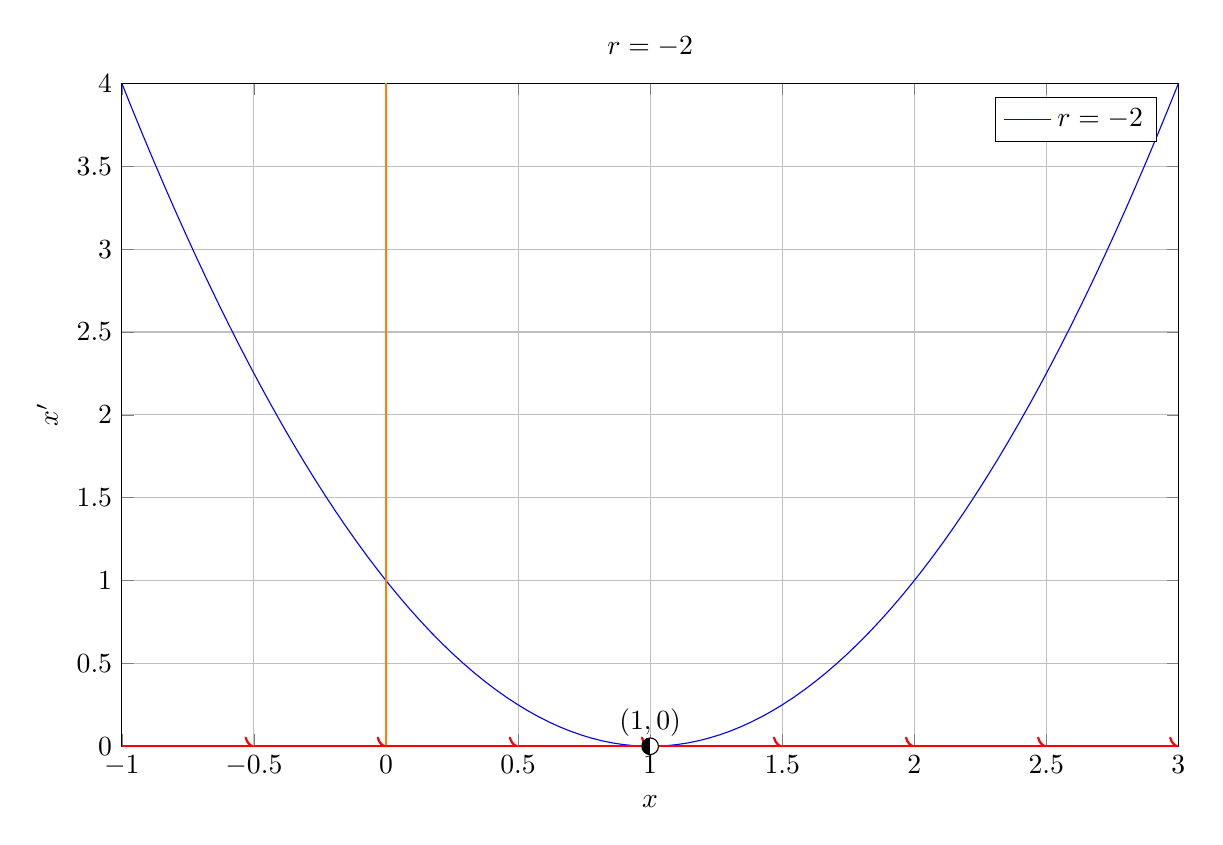
\begin{tikzpicture}
		\begin{axis}[
			title = {$r=-2$},
			xlabel = {$x$},
			ylabel = {$x'$},
			xmin = -1, xmax = 3,
			ymin = 0, ymax = 4,
			grid = major,
			width=15cm,
			height=10cm,
			]

			% when r=-2
			\addplot[blue, domain=-1:3, samples=100] {1-2*x+x^2};
			% add horizontal line x=0
			\addplot[orange, domain=-3:3, samples=100] {0};
			% add vertical line y=0
			\addplot[orange, domain=-3:3, samples=100] coordinates {(0,0) (0,6)};

			% add half circle at (1,0)
			\addplot[mark=halfcircle*, mark options={rotate=90}, mark size=3pt] coordinates {(1, 0)} node[above]{$(1,0)$};

			% draw vector form (-3,0) to (-2.5,0) and change the arrow to thick
			\addplot[->, thick, color=red] coordinates {(-3,0) (-2.5,0)};
			% draw vector form (-2.5,0) to (-2,0) and change the arrow to thick
			\addplot[->, thick, color=red] coordinates {(-2.5,0) (-2,0)};
			% draw vector form (-2,0) to (-1.5,0) and change the arrow to thick
			\addplot[->, thick, color=red] coordinates {(-2,0) (-1.5,0)};
			% draw vector form (-1.5,0) to (-1,0) and change the arrow to thick
			\addplot[->, thick, color=red] coordinates {(-1.5,0) (-1,0)};
			% draw vector form (-1,0) to (-0.5,0) and change the arrow to thick
			\addplot[->, thick, color=red] coordinates {(-1,0) (-0.5,0)};
			% draw vector form (-0.5,0) to (0,0) and change the arrow to thick
			\addplot[->, thick, color=red] coordinates {(-0.5,0) (0,0)};
			% draw vector form (0,0) to (0.5,0) and change the arrow to thick
			\addplot[->, thick, color=red] coordinates {(0,0) (0.5,0)};
			% draw vector form (0.5,0) to (1,0) and change the arrow to thick
			\addplot[->, thick, color=red] coordinates {(0.5,0) (1,0)};
			% draw vector form (1,0) to (1.5,0) and change the arrow to thick
			\addplot[->, thick, color=red] coordinates {(1,0) (1.5,0)};
			% draw vector form (1.5,0) to (2,0) and change the arrow to thick
			\addplot[->, thick, color=red] coordinates {(1.5,0) (2,0)};
			% draw vector form (2,0) to (2.5,0) and change the arrow to thick
			\addplot[->, thick, color=red] coordinates {(2,0) (2.5,0)};
			% draw vector form (2.5,0) to (3,0) and change the arrow to thick
			\addplot[->, thick, color=red] coordinates {(2.5,0) (3,0)};
			
			\legend{$r=-2$}
			\end{axis}
		\end{tikzpicture}

	\item When $r<-2$, we can sketch the vector field as below:

		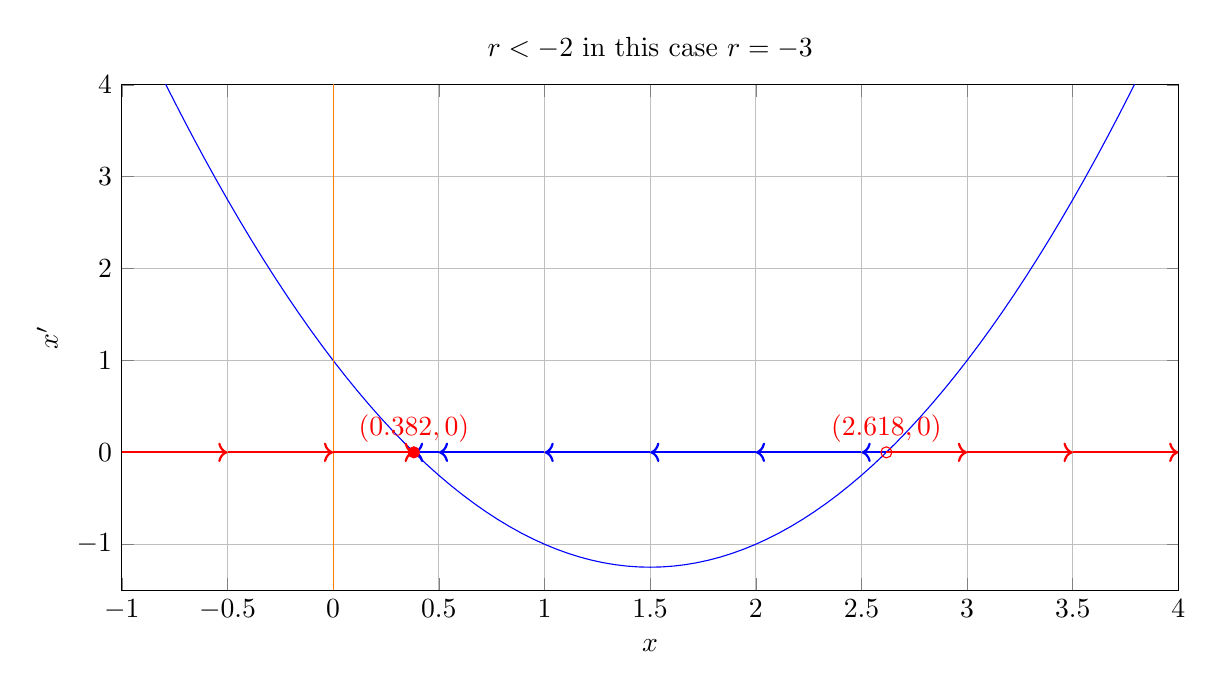
\begin{tikzpicture}
		\begin{axis}[
			title = {$r<-2$ in this case $r=-3$},
			xlabel = {$x$},
			ylabel = {$x'$},
			xmin = -1, xmax = 4,
			ymin = -1.5, ymax = 4 ,
			grid = major,
			width=15cm,
			height=8cm,
			]

			% when r=-3
			\addplot[blue, domain=-1.5:4, samples=100] {1-3*x+x^2};
			% add horizontal line x=0
			\addplot[orange, domain=-3:4, samples=100] {0};
			% add vertical line y=0
			\addplot[orange, domain=-3:4, samples=100] coordinates {(0,-1.5) (0,6)};

			% add point at (0.382,0)
			\addplot[only marks, mark=*, mark size=2pt, color=red] coordinates {(0.382,0)} node[above]{$(0.382,0)$};
			% add hollow point at (2.618,0) with label
			\addplot[only marks, mark=o, mark size=2pt, color=red] coordinates {(2.618,0)} node[above]{$(2.618,0)$};

			% draw vector from (-1,0) to (-0.5,0) and change the arrow to thick
			\addplot[->, thick, color=red] coordinates {(-1,0) (-0.5,0)};
			% draw vector from (-0.5,0) to (0,0) and change the arrow to thick
			\addplot[->, thick, color=red] coordinates {(-0.5,0) (0,0)};
			% draw vector from (0,0) to (0.382,0) and change the arrow to thick
			\addplot[->, thick, color=red] coordinates {(0,0) (0.382,0)};
			% draw vector from (2.618,0) to (3,0) and change the arrow to thick
			\addplot[->, thick, color=red] coordinates {(2.618,0) (3,0)};
			% draw vector from (3,0) to (3.5,0) and change the arrow to thick
			\addplot[->, thick, color=red] coordinates {(3,0) (3.5,0)};
			% draw vector from (3.5,0) to (4,0) and change the arrow to thick
			\addplot[->, thick, color=red] coordinates {(3.5,0) (4,0)};

			% draw vector from (2.618,0) to (2.5,0) and change the arrow to thick
			\addplot[->, thick, color=blue] coordinates {(2.618,0) (2.5,0)};
			% draw vector from (2.5,0) to (2,0) and change the arrow to thick
			\addplot[->, thick, color=blue] coordinates {(2.5,0) (2,0)};
			% draw vector from (2,0) to (1.5,0) and change the arrow to thick
			\addplot[->, thick, color=blue] coordinates {(2,0) (1.5,0)};
			% draw vector from (1.5,0) to (1,0) and change the arrow to thick
			\addplot[->, thick, color=blue] coordinates {(1.5,0) (1,0)};
			% draw vector from (1,0) to (0.5,0) and change the arrow to thick
			\addplot[->, thick, color=blue] coordinates {(1,0) (0.5,0)};
			% draw vector from (0.5,0) to (0.382,0) and change the arrow to thick
			\addplot[->, thick, color=blue] coordinates {(0.5,0) (0.382,0)};


			\end{axis}
		\end{tikzpicture}

The bifurcation diagram of $x$ vs. $r$ is below:

		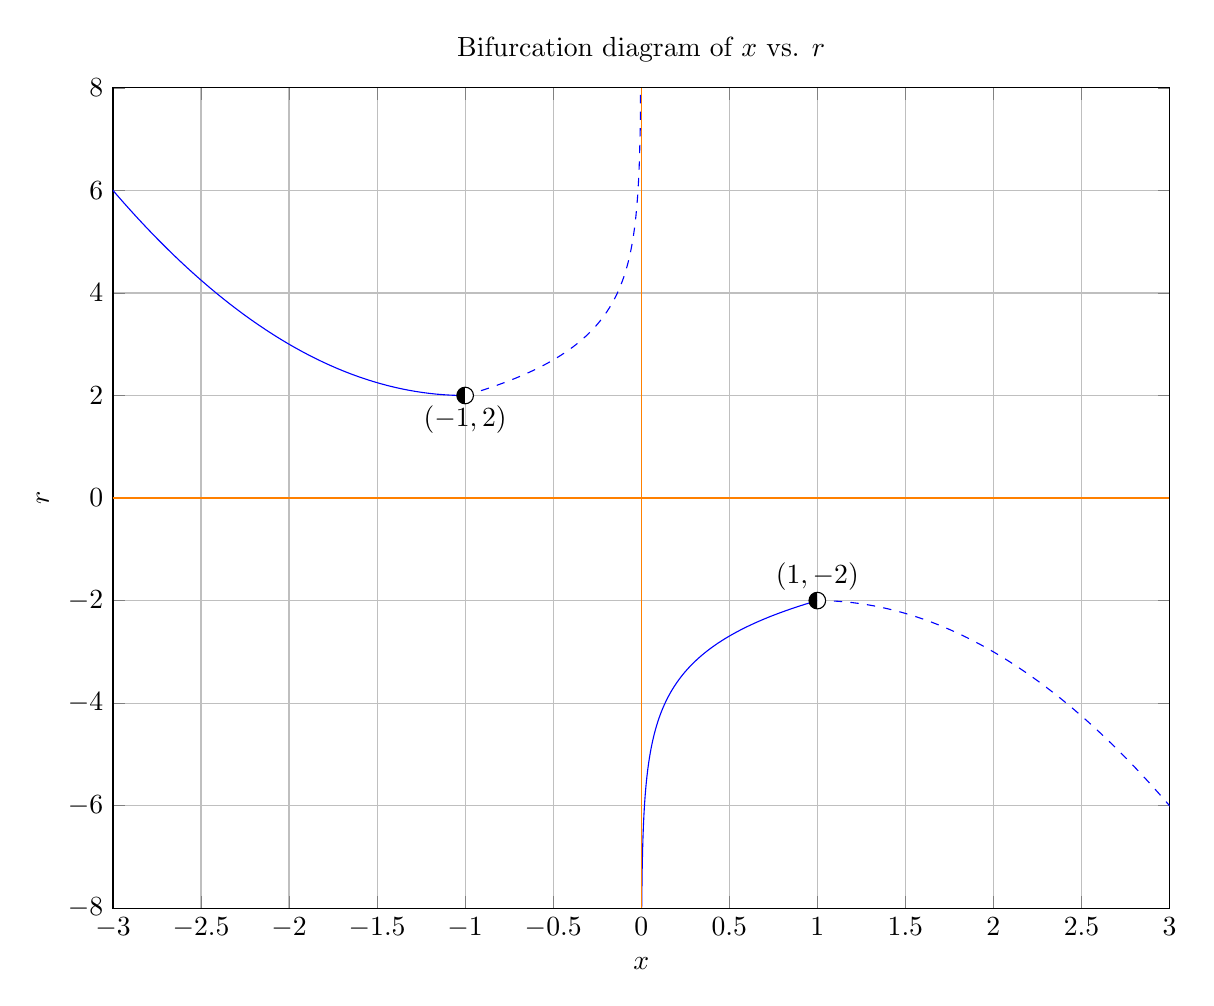
\begin{tikzpicture}
		\begin{axis}[
			title = {Bifurcation diagram of $x$ vs. $r$},
			xlabel = {$x$},
			ylabel = {$r$},
			xmin = -3, xmax = 3,
			ymin = -8, ymax = 8,
			grid = major,
			width=15cm,
			height=12cm,
			]
			
			% log_e(x)-2 where x \in [0,1]
			\addplot[blue, domain=0:1, samples=400] {ln(x)-2};
			% -\left(x-1\right)^{2}-2 where x \in [1,5] with dashed line
			\addplot[blue, domain=1:5, samples=100, dashed] {-(x-1)^2-2};
			% -\ln\left(-x\right)+2 where x \in [-1,0] with dashed line
			\addplot[blue, domain=-1:0, samples=200, dashed] {-ln(-x)+2};
			% \left(x+1\right)^{2}+2 where x \in [-5,-1]
			\addplot[blue, domain=-5:-1, samples=100] {(x+1)^2+2};
			
		
			% add horizontal line x=0
			\addplot[orange, domain=-3:3, samples=100] {0};
			% add vertical line y=0
			\addplot[orange, domain=-3:3, samples=100] coordinates {(0,-8) (0,8)};

			% add half circle at (1,-2)
			\addplot[mark=halfcircle*, mark options={rotate=90}, mark size=3pt] coordinates {(1, -2)} node[above]{$(1,-2)$};
			% add half circle at (-1,2)
			\addplot[mark=halfcircle*, mark options={rotate=90}, mark size=3pt] coordinates {(-1, 2)} node[below]{$(-1,2)$};

		\end{axis}
		\end{tikzpicture}

\end{enumerate}



\section*{Problem 2}
For ODE $x'=rx-\ln(1+x)$, we will find the Bifurcation diagram.
\begin{enumerate}[(a)]
	\item When $1<r$, we have vector field below:

		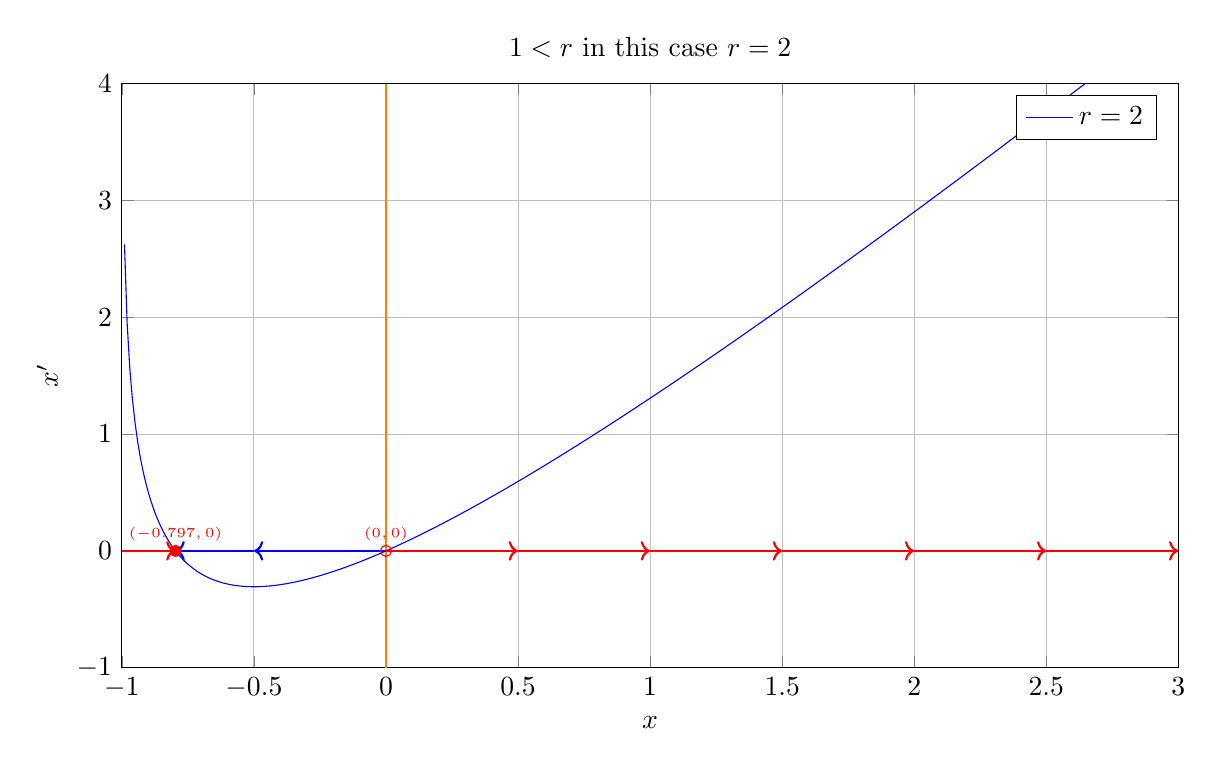
\begin{tikzpicture}
		\begin{axis}[
			title = {$1<r$ in this case $r=2$},
			xlabel = {$x$},
			ylabel = {$x'$},
			xmin = -1, xmax = 3,
			ymin = -1, ymax = 4,
			grid = major,
			width=15cm,
			height=9cm,
			]

			% when r=2
			\addplot[blue, domain=-1:3, samples=400] {2*x-ln(1+x)};
			% add horizontal line x=0
			\addplot[orange, domain=-1:3, samples=100] {0};
			% add vertical line y=0
			\addplot[orange, domain=-1:3, samples=100] coordinates {(0,-1) (0,4)};

			% add point at (-0.797,0)
			\addplot[only marks, mark=*, mark size=2pt, color=red] coordinates {(-0.797,0)} node[above, font=\tiny]{$(-0.797,0)$};
			% add hollow point at (0,0) with label
			\addplot[only marks, mark=o, mark size=2pt, color=red] coordinates {(0,0)} node[above, font=\tiny]{$(0,0)$};

			% draw vector from (-1,0) to (-0.797,0) and change the arrow to thick
			\addplot[->, thick, color=red] coordinates {(-1,0) (-0.797,0)};
			% draw vector from (0,0) to (0.5,0) and change the arrow to thick
			\addplot[->, thick, color=red] coordinates {(0,0) (0.5,0)};
			% draw vector from (0.5,0) to (1,0) and change the arrow to thick
			\addplot[->, thick, color=red] coordinates {(0.5,0) (1,0)};
			% draw vector from (1,0) to (1.5,0) and change the arrow to thick
			\addplot[->, thick, color=red] coordinates {(1,0) (1.5,0)};
			% draw vector from (1.5,0) to (2,0) and change the arrow to thick
			\addplot[->, thick, color=red] coordinates {(1.5,0) (2,0)};
			% draw vector from (2,0) to (2.5,0) and change the arrow to thick
			\addplot[->, thick, color=red] coordinates {(2,0) (2.5,0)};
			% draw vector from (2.5,0) to (3,0) and change the arrow to thick
			\addplot[->, thick, color=red] coordinates {(2.5,0) (3,0)};
			
			% draw vector from (0,0) to (-0.5,0) and change the arrow to thick
			\addplot[->, thick, color=blue] coordinates {(0,0) (-0.5,0)};
			% draw vector from (-0.5,0) to (-0.797,0) and change the arrow to thick
			\addplot[->, thick, color=blue] coordinates {(-0.5,0) (-0.797,0)};

		
		\legend{$r=2$}
		\end{axis}
		\end{tikzpicture}

	\item When $r=1$, we have vector field below:

		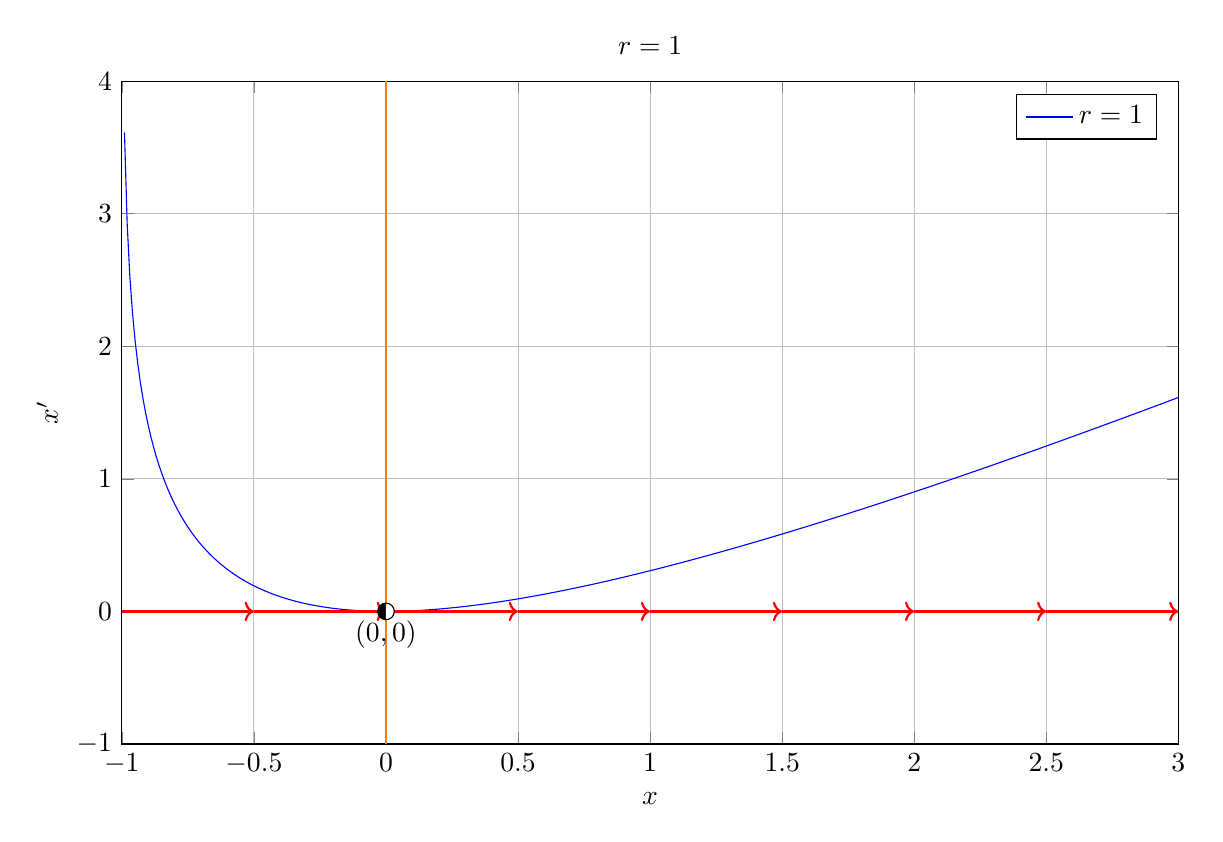
\begin{tikzpicture}
		\begin{axis}[
			title = {$r=1$},
			xlabel = {$x$},
			ylabel = {$x'$},
			xmin = -1, xmax = 3,
			ymin = -1, ymax = 4,
			grid = major,
			width=15cm,
			height=10cm,
			]
			
			% when r=1
			\addplot[blue, domain=-1:3, samples=400] {x-ln(1+x)};
			% add horizontal line x=0	
			\addplot[orange, domain=-1:3, samples=100] {0};
			% add vertical line y=0
			\addplot[orange, domain=-1:3, samples=100] coordinates {(0,-1) (0,4)};
			
			% add half circle at (0,0)
			\addplot[mark=halfcircle*, mark options={rotate=90}, mark size=3pt] coordinates {(0, 0)} node[below]{$(0,0)$};

			% draw vector from (-1,0) to (-0.5,0) and change the arrow to thick
			\addplot[->, thick, color=red] coordinates {(-1,0) (-0.5,0)};
			% draw vector from (-0.5,0) to (0,0) and change the arrow to thick
			\addplot[->, thick, color=red] coordinates {(-0.5,0) (0,0)};
			% draw vector from (0,0) to (0.5,0) and change the arrow to thick
			\addplot[->, thick, color=red] coordinates {(0,0) (0.5,0)};
			% draw vector from (0.5,0) to (1,0) and change the arrow to thick
			\addplot[->, thick, color=red] coordinates {(0.5,0) (1,0)};
			% draw vector from (1,0) to (1.5,0) and change the arrow to thick
			\addplot[->, thick, color=red] coordinates {(1,0) (1.5,0)};
			% draw vector from (1.5,0) to (2,0) and change the arrow to thick
			\addplot[->, thick, color=red] coordinates {(1.5,0) (2,0)};
			% draw vector from (2,0) to (2.5,0) and change the arrow to thick
			\addplot[->, thick, color=red] coordinates {(2,0) (2.5,0)};
			% draw vector from (2.5,0) to (3,0) and change the arrow to thick
			\addplot[->, thick, color=red] coordinates {(2.5,0) (3,0)};

			\legend{$r=1$}
			\end{axis}
		\end{tikzpicture}
	
	\item When $0<r<1$, we have vector field below:

		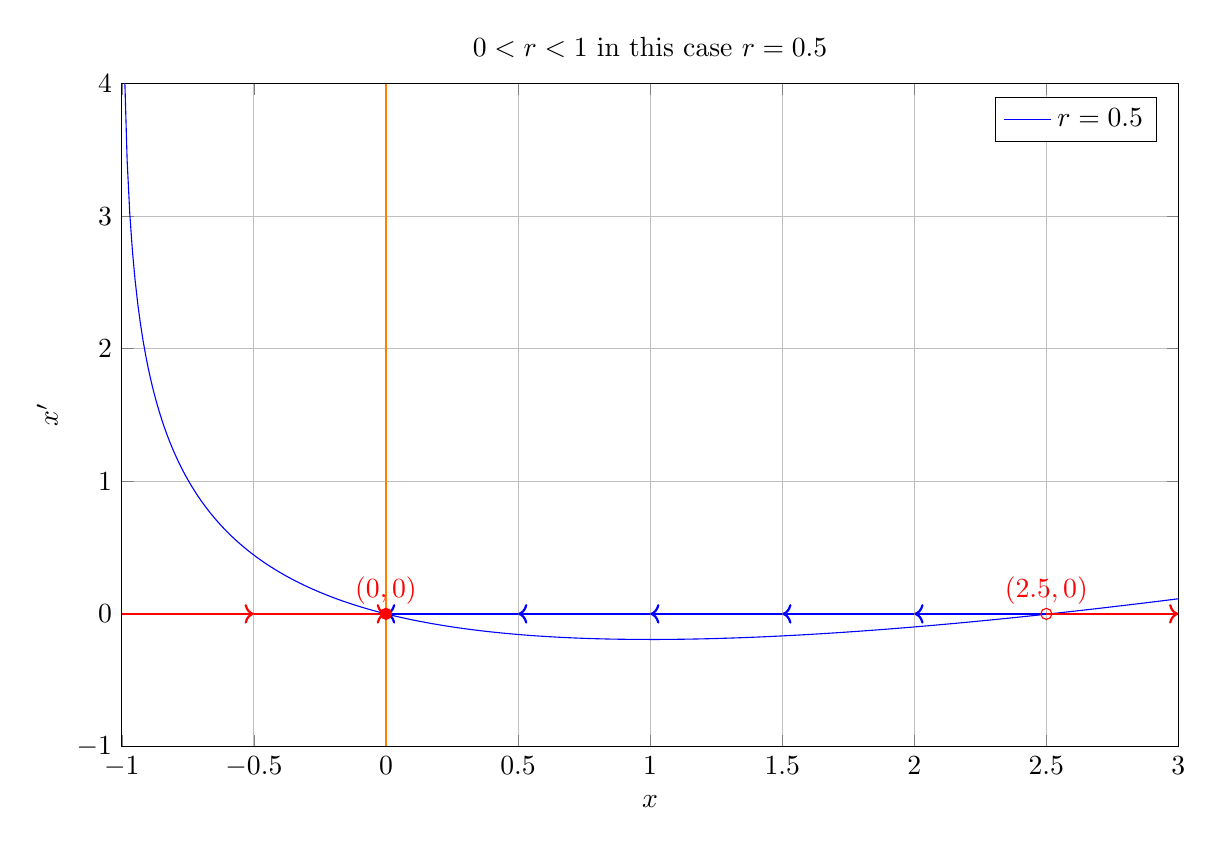
\begin{tikzpicture}
		\begin{axis}[
			title = {$0<r<1$ in this case $r=0.5$},
			xlabel = {$x$},
			ylabel = {$x'$},
			xmin = -1, xmax = 3,
			ymin = -1, ymax = 4,
			grid = major,
			width=15cm,
			height=10cm,
			]

			% when r=0.5
			\addplot[blue, domain=-1:3, samples=400] {0.5*x-ln(1+x)};
			% add horizontal line x=0
			\addplot[orange, domain=-1:3, samples=100] {0};
			% add vertical line y=0
			\addplot[orange, domain=-1:3, samples=100] coordinates {(0,-1) (0,4)};

			% add point at (0,0)
			\addplot[only marks, mark=*, mark size=2pt, color=red] coordinates {(0,0)} node[above]{$(0,0)$};
			% add hollow point at (2.5,0) with label
			\addplot[only marks, mark=o, mark size=2pt, color=red] coordinates {(2.5,0)} node[above]{$(2.5,0)$};

			% draw vector from (-1,0) to (-0.5,0) and change the arrow to thick
			\addplot[->, thick, color=red] coordinates {(-1,0) (-0.5,0)};
			% draw vector from (-0.5,0) to (0,0) and change the arrow to thick
			\addplot[->, thick, color=red] coordinates {(-0.5,0) (0,0)};
			% draw vector from (2.5,0) to (3,0) and change the arrow to thick
			\addplot[->, thick, color=red] coordinates {(2.5,0) (3,0)};

			% draw vector from (0.5,0) to (0,0) and change the arrow to thick
			\addplot[->, thick, color=blue] coordinates {(0.5,0) (0,0)};	
			% draw vector from (1,0) to (0.5,0) and change the arrow to thick
			\addplot[->, thick, color=blue] coordinates {(1,0) (0.5,0)};
			% draw vector from (1.5,0) to (1,0) and change the arrow to thick
			\addplot[->, thick, color=blue] coordinates {(1.5,0) (1,0)};
			% draw vector from (2,0) to (1.5,0) and change the arrow to thick
			\addplot[->, thick, color=blue] coordinates {(2,0) (1.5,0)};
			% draw vector from (2.5,0) to (2,0) and change the arrow to thick
			\addplot[->, thick, color=blue] coordinates {(2.5,0) (2,0)};

			\legend{$r=0.5$}
			\end{axis}
		\end{tikzpicture}

	\item When $r \leq 0$, we have vector field below:

		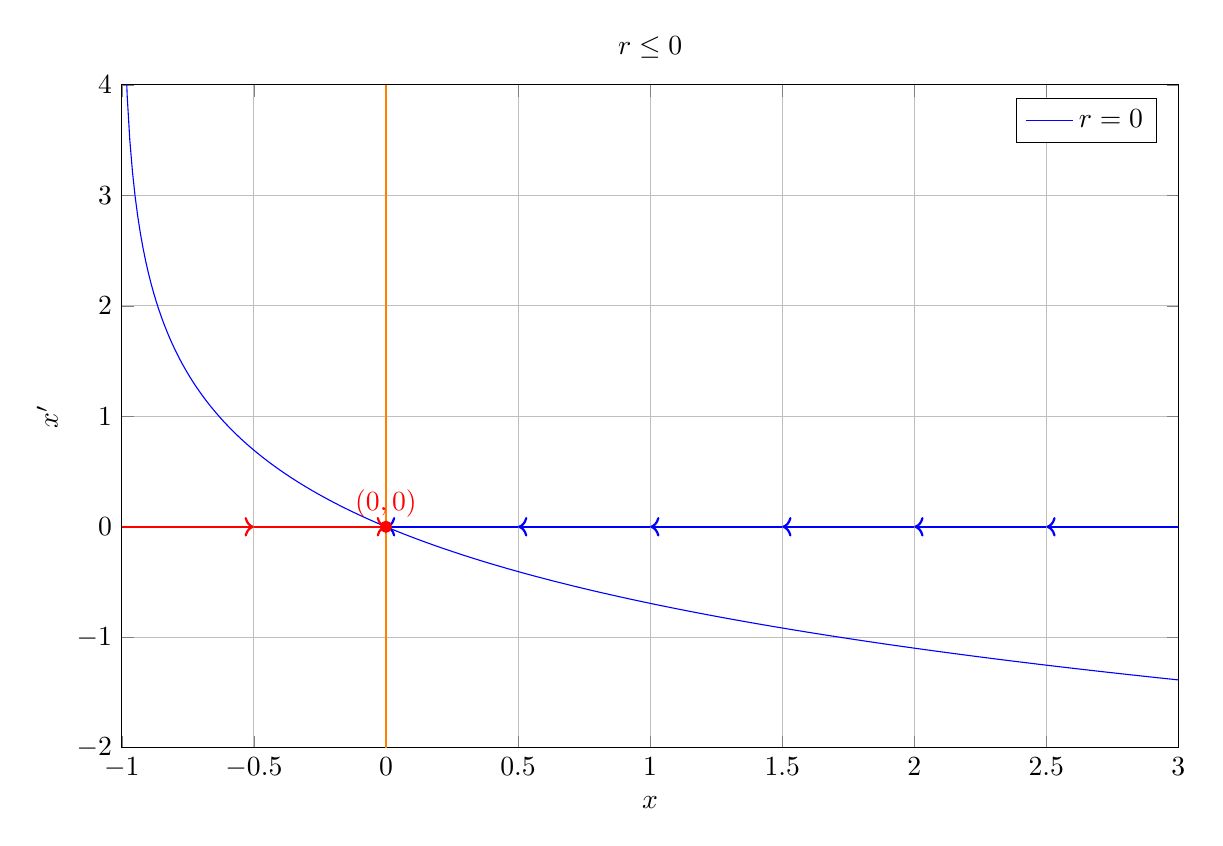
\begin{tikzpicture}
		\begin{axis}[
			title = {$r \leq 0$},
			xlabel = {$x$},
			ylabel = {$x'$},
			xmin = -1, xmax = 3,
			ymin = -2, ymax = 4,
			grid = major,
			width=15cm,
			height=10cm,
			]

			% when r=0
			\addplot[blue, domain=-1:3, samples=400] {-ln(1+x)};
			% add horizontal line x=0
			\addplot[orange, domain=-1:3, samples=100] {0};
			% add vertical line y=0
			\addplot[orange, domain=-1:3, samples=100] coordinates {(0,-2) (0,4)};

			% add point at (0,0)
			\addplot[only marks, mark=*, mark size=2pt, color=red] coordinates {(0,0)} node[above]{$(0,0)$};
			
			% draw vector from (-1,0) to (-0.5,0) and change the arrow to thick
			\addplot[->, thick, color=red] coordinates {(-1,0) (-0.5,0)};
			% draw vector from (-0.5,0) to (0,0) and change the arrow to thick
			\addplot[->, thick, color=red] coordinates {(-0.5,0) (0,0)};
			
			% draw vector from (0.5,0) to (0,0) and change the arrow to thick
			\addplot[->, thick, color=blue] coordinates {(0.5,0) (0,0)};
			% draw vector from (1,0) to (0.5,0) and change the arrow to thick
			\addplot[->, thick, color=blue] coordinates {(1,0) (0.5,0)};
			% draw vector from (1.5,0) to (1,0) and change the arrow to thick
			\addplot[->, thick, color=blue] coordinates {(1.5,0) (1,0)};
			% draw vector from (2,0) to (1.5,0) and change the arrow to thick
			\addplot[->, thick, color=blue] coordinates {(2,0) (1.5,0)};
			% draw vector from (2.5,0) to (2,0) and change the arrow to thick
			\addplot[->, thick, color=blue] coordinates {(2.5,0) (2,0)};
			% draw vector from (3,0) to (2.5,0) and change the arrow to thick
			\addplot[->, thick, color=blue] coordinates {(3,0) (2.5,0)};

			\legend{$r=0$}


			\end{axis}
		\end{tikzpicture}
		
\end{enumerate}

The bifurcation diagram of $x$ vs. $r$ is below:

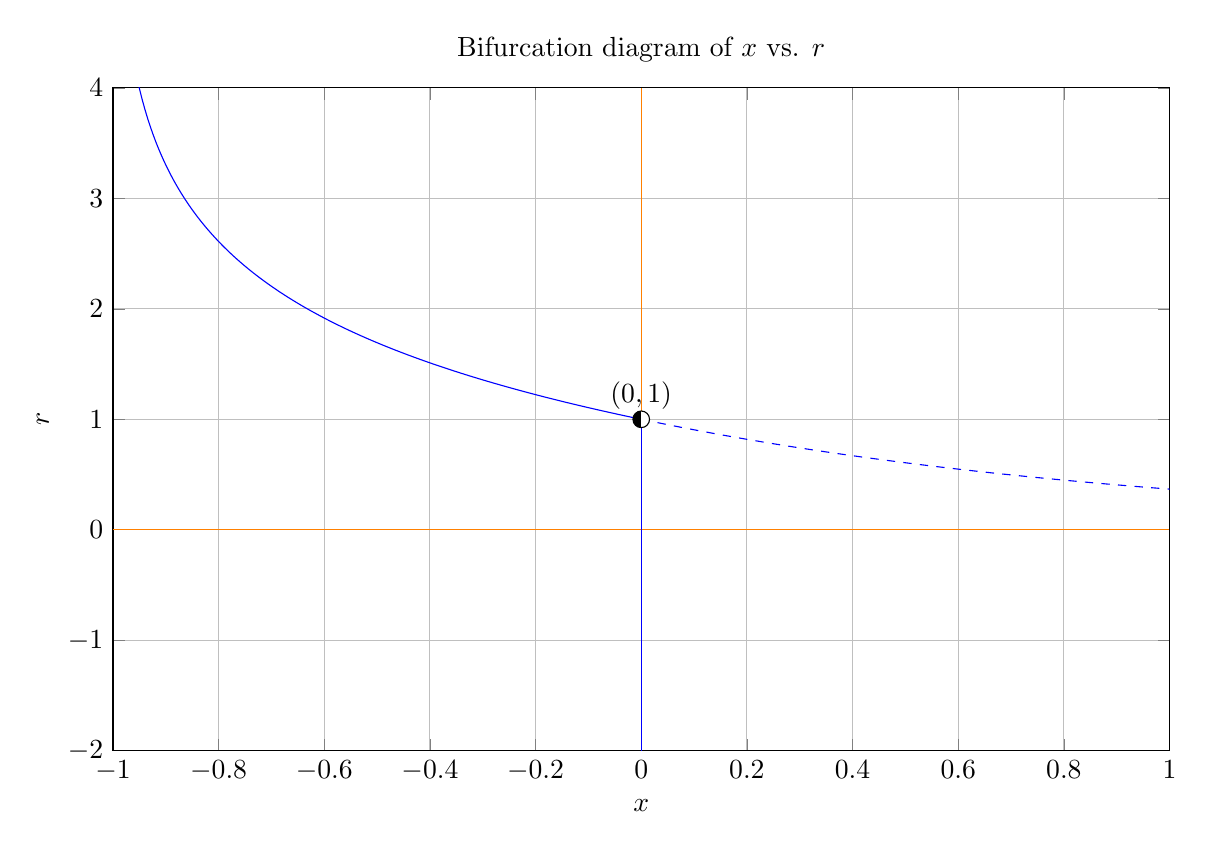
\begin{tikzpicture}
\begin{axis}[
	title = {Bifurcation diagram of $x$ vs. $r$},
	xlabel = {$x$},
	ylabel = {$r$},
	xmin = -1, xmax = 1,
	ymin = -2, ymax = 4,
	grid = major,
	width=15cm,
	height=10cm,
	]

	% -\ln\left(x+1\right)+1 where x \in [-1,0]
	\addplot[blue, domain=-1:0, samples=200] {-ln(x+1)+1};
	% e^{-x} where x \in [0,3] with dash line
	\addplot[blue, domain=0:3, samples=200, dashed] {e^(-x)};
	% add horizontal line x=0
	\addplot[orange, domain=-1:1, samples=100] {0};
	% add vertical line y=0
	\addplot[orange, domain=-1:1, samples=100] coordinates {(0,-2) (0,4)};
	% add vertical line y=0 from x=1 to x=-2
	\addplot[blue, domain=-1:3, samples=100] coordinates {(0,1) (0,-2)};
	
	% add half circle at (0,1)
	\addplot[mark=halfcircle*, mark options={rotate=90}, mark size=3pt] coordinates {(0, 1)} node[above]{$(0,1)$};


	\end{axis}
\end{tikzpicture}


\section*{Problem 3}
For ODE $x'=x+rx/(1+x^2)$, we will find the Bifurcation diagram.

\begin{enumerate}[(a)]
	\item When $r \geq -1$, we have vector field below:
	
	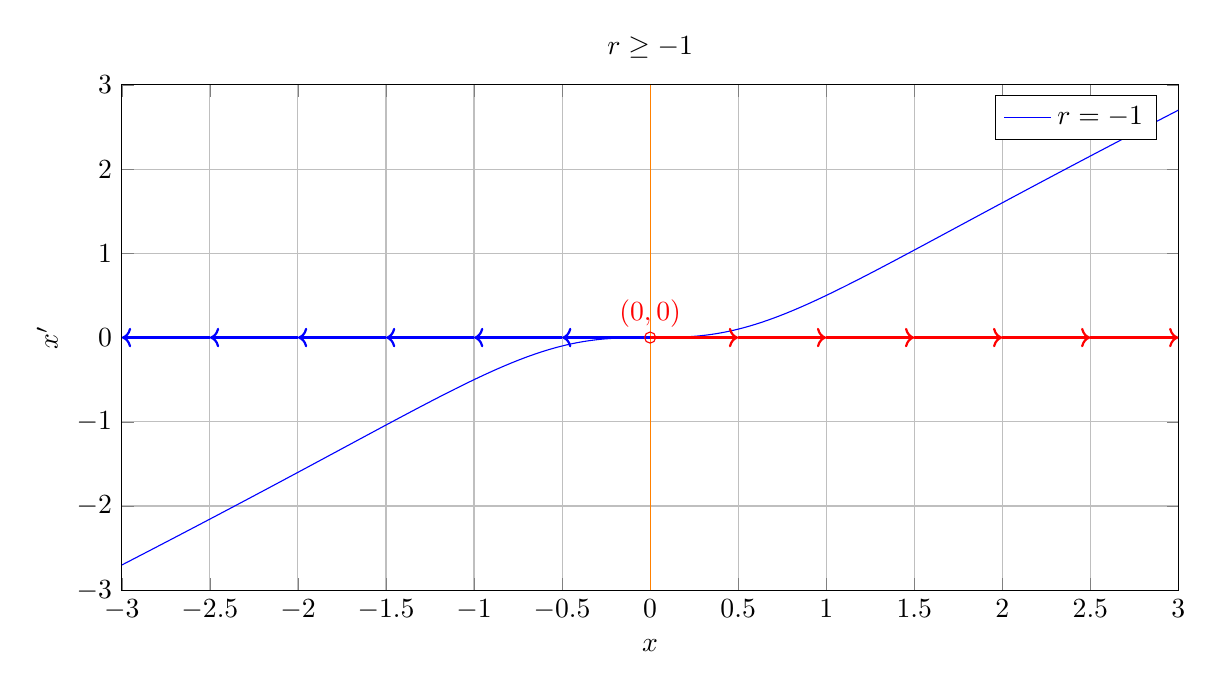
\begin{tikzpicture}
	\begin{axis}[
		title = {$r \geq -1$},
		xlabel = {$x$},
		ylabel = {$x'$},
		xmin = -3, xmax = 3,
		ymin = -3, ymax = 3,
		grid = major,
		width=15cm,
		height=8cm,
		]

		% when r=-1
		\addplot[blue, domain=-3:3, samples=400] {x-x/(1+x^2)};
		% add horizontal line x=0
		\addplot[orange, domain=-3:3, samples=100] {0};
		% add vertical line y=0
		\addplot[orange, domain=-3:3, samples=100] coordinates {(0,-3) (0,3)};
		
		% add hollow point at (0,0)
		\addplot[only marks, mark=o, mark size=2pt, color=red] coordinates {(0,0)} node[above]{$(0,0)$};

		% draw vector from (-2.5,0) to (-3,0) and change the arrow to thick
		\addplot[->, thick, color=blue] coordinates {(-2.5,0) (-3,0)};
		% draw vector from (-2,0) to (-2.5,0) and change the arrow to thick
		\addplot[->, thick, color=blue] coordinates {(-2,0) (-2.5,0)};
		% draw vector from (-1.5,0) to (-2,0) and change the arrow to thick
		\addplot[->, thick, color=blue] coordinates {(-1.5,0) (-2,0)};
		% draw vector from (-1,0) to (-1.5,0) and change the arrow to thick
		\addplot[->, thick, color=blue] coordinates {(-1,0) (-1.5,0)};
		% draw vector from (-0.5,0) to (-1,0) and change the arrow to thick
		\addplot[->, thick, color=blue] coordinates {(-0.5,0) (-1,0)};
		% draw vector from (0,0) to (-0.5,0) and change the arrow to thick
		\addplot[->, thick, color=blue] coordinates {(0,0) (-0.5,0)};

		% draw vector from (0,0) to (0.5,0) and change the arrow to thick
		\addplot[->, thick, color=red] coordinates {(0,0) (0.5,0)};
		% draw vector from (0.5,0) to (1,0) and change the arrow to thick
		\addplot[->, thick, color=red] coordinates {(0.5,0) (1,0)};
		% draw vector from (1,0) to (1.5,0) and change the arrow to thick
		\addplot[->, thick, color=red] coordinates {(1,0) (1.5,0)};
		% draw vector from (1.5,0) to (2,0) and change the arrow to thick
		\addplot[->, thick, color=red] coordinates {(1.5,0) (2,0)};
		% draw vector from (2,0) to (2.5,0) and change the arrow to thick
		\addplot[->, thick, color=red] coordinates {(2,0) (2.5,0)};
		% draw vector from (2.5,0) to (3,0) and change the arrow to thick
		\addplot[->, thick, color=red] coordinates {(2.5,0) (3,0)};


		\legend{$r=-1$}
		\end{axis}
	\end{tikzpicture}
		
	\item When $r<-1$, we have vector field below:

	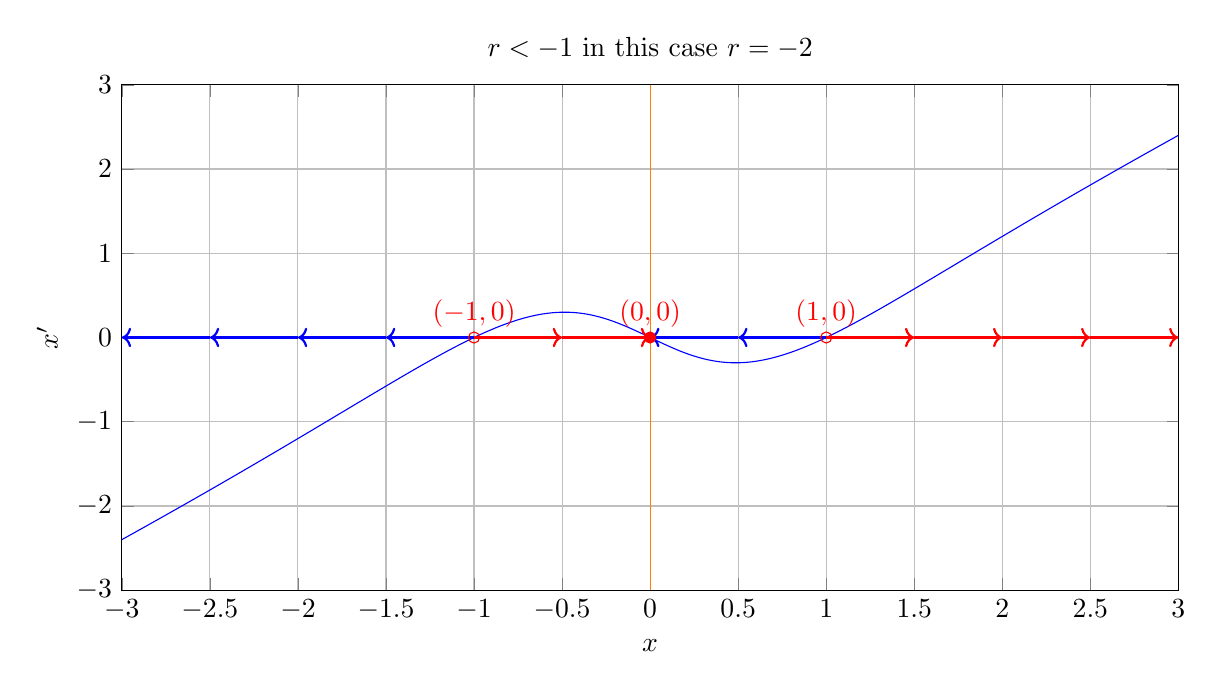
\begin{tikzpicture}
	\begin{axis}[
		title = {$r<-1$ in this case $r=-2$},
		xlabel = {$x$},
		ylabel = {$x'$},
		xmin = -3, xmax = 3,
		ymin = -3, ymax = 3,
		grid = major,
		width=15cm,
		height=8cm,
		]

		% when r=-2
		\addplot[blue, domain=-3:3, samples=400] {x-2*x/(1+x^2)};
		% add horizontal line x=0
		\addplot[orange, domain=-3:3, samples=100] {0};
		% add vertical line y=0
		\addplot[orange, domain=-3:3, samples=100] coordinates {(0,-3) (0,3)};
		
		% add point at (0,0)
		\addplot[only marks, mark=*, mark size=2pt, color=red] coordinates {(0,0)} node[above]{$(0,0)$};
		% add hollow point at (-1,0) with label
		\addplot[only marks, mark=o, mark size=2pt, color=red] coordinates {(-1,0)} node[above]{$(-1,0)$};
		% add hollow point at (1,0) with label
		\addplot[only marks, mark=o, mark size=2pt, color=red] coordinates {(1,0)} node[above]{$(1,0)$};
		
		% draw vector from (-2.5,0) to (-3,0) and change the arrow to thick
		\addplot[->, thick, color=blue] coordinates {(-2.5,0) (-3,0)};
		% draw vector from (-2,0) to (-2.5,0) and change the arrow to thick
		\addplot[->, thick, color=blue] coordinates {(-2,0) (-2.5,0)};
		% draw vector from (-1.5,0) to (-2,0) and change the arrow to thick
		\addplot[->, thick, color=blue] coordinates {(-1.5,0) (-2,0)};
		% draw vector from (-1,0) to (-1.5,0) and change the arrow to thick
		\addplot[->, thick, color=blue] coordinates {(-1,0) (-1.5,0)};
		% draw vector from (0.5,0) to (0,0) and change the arrow to thick
		\addplot[->, thick, color=blue] coordinates {(0.5,0) (0,0)};
		% draw vector from (1,0) to (0.5,0) and change the arrow to thick
		\addplot[->, thick, color=blue] coordinates {(1,0) (0.5,0)};

		% draw vector from (-1,0) to (-0.5,0) and change the arrow to thick
		\addplot[->, thick, color=red] coordinates {(-1,0) (-0.5,0)};
		% draw vector from (-0.5,0) to (0,0) and change the arrow to thick
		\addplot[->, thick, color=red] coordinates {(-0.5,0) (0,0)};
		% draw vector from (1,0) to (1.5,0) and change the arrow to thick
		\addplot[->, thick, color=red] coordinates {(1,0) (1.5,0)};	
		% draw vector from (1.5,0) to (2,0) and change the arrow to thick
		\addplot[->, thick, color=red] coordinates {(1.5,0) (2,0)};
		% draw vector from (2,0) to (2.5,0) and change the arrow to thick
		\addplot[->, thick, color=red] coordinates {(2,0) (2.5,0)};
		% draw vector from (2.5,0) to (3,0) and change the arrow to thick
		\addplot[->, thick, color=red] coordinates {(2.5,0) (3,0)};


	\end{axis}
	\end{tikzpicture}

	\item From the behavior of the vector field, we can see that the bifurcation point is $r=-1$. When $r>-1$, the fixed point is $x=0$ and it is unstable. When $r<-1$, the fixed point is $x=0$ and it is stable and occurs two unstable fixed points $x=\pm \sqrt{-r-1}$. That is a classic subcritical pitchfork bifurcation.
\end{enumerate}

The subcritical pitchfork bifurcation diagram of $x$ vs. $r$ is below:

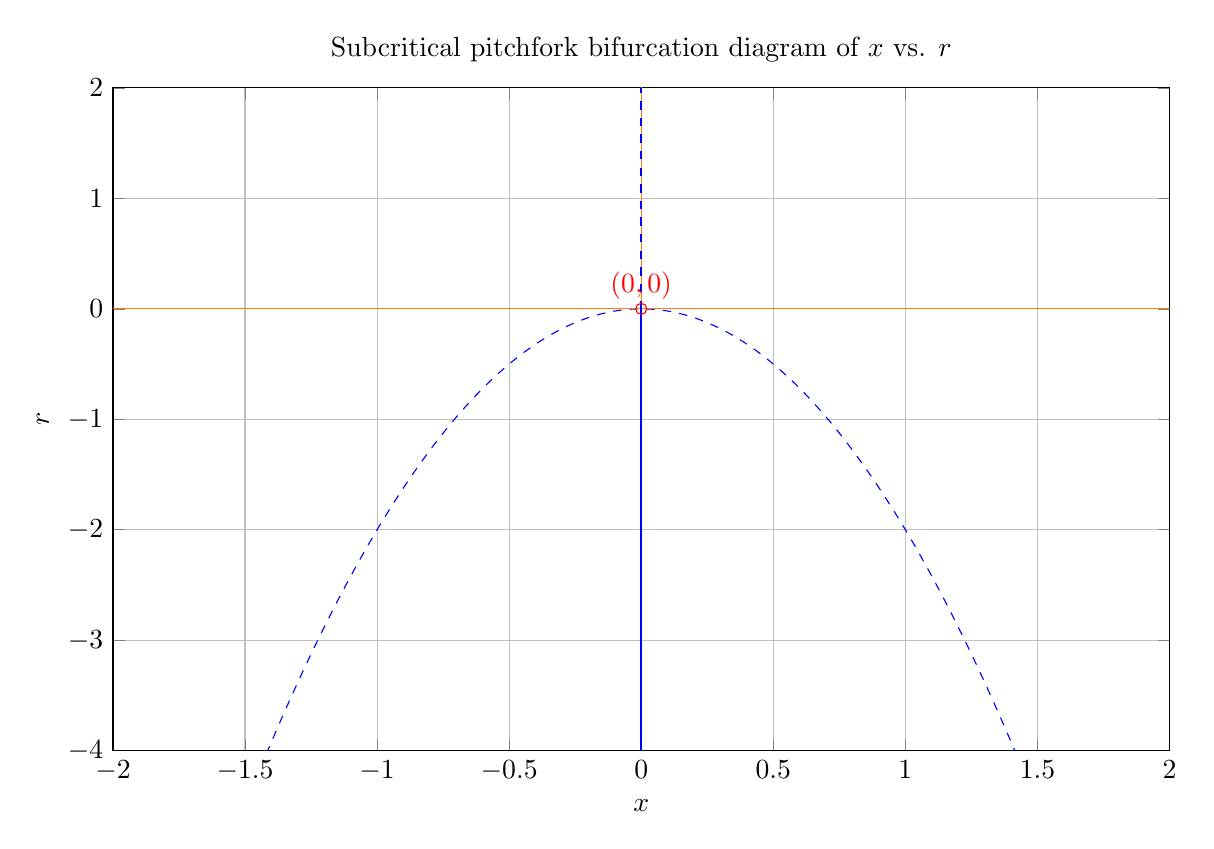
\begin{tikzpicture}
\begin{axis}[
	title = {Subcritical pitchfork bifurcation diagram of $x$ vs. $r$},
	xlabel = {$x$},
	ylabel = {$r$},
	xmin = -2, xmax = 2,
	ymin = -4, ymax = 2,
	grid = major,
	width=15cm,
	height=10cm,
	]

	% -\left(\sqrt{2}x\right)^{2} where x \in [-1,1] with dash line
	\addplot[blue, domain=-2:2, samples=200, dashed] {-(sqrt(2)*x)^2};
	% add horizontal line x=0
	\addplot[orange, domain=-2:2, samples=100] {0};
	% add vertical line y=0
	\addplot[orange, domain=-2:2, samples=100] coordinates {(0,-4) (0,4)};
	% add vertical line y=0 from x=0 to x=2 dash line
	\addplot[blue, domain=-2:2, samples=100, dashed, thick] coordinates {(0,0) (0,2)};
	% add vertical line y=0 from x=0 to x=-4 
	\addplot[blue, domain=-2:2, samples=100, thick] coordinates {(0,0) (0,-4)};

	% add hollow point at (0,0)
	\addplot[only marks, mark=o, mark size=2pt, color=red] coordinates {(0,0)} node[above]{$(0,0)$};

	\end{axis}
\end{tikzpicture}


\section*{Problem 4}
Consider the ODE $x'=rx+x^3-x^5$.

\begin{enumerate}[(a)]
	\item Find the potential function $V(x)$ for the ODE.
	\[V(x)=\int -x'dx=\int (-rx-x^3+x^5)dx=-\frac{r}{2}x^2-\frac{1}{4}x^4+\frac{1}{6}x^6+C.\]
	Then the plot of $V(x)$ is below (When $C=0$):

	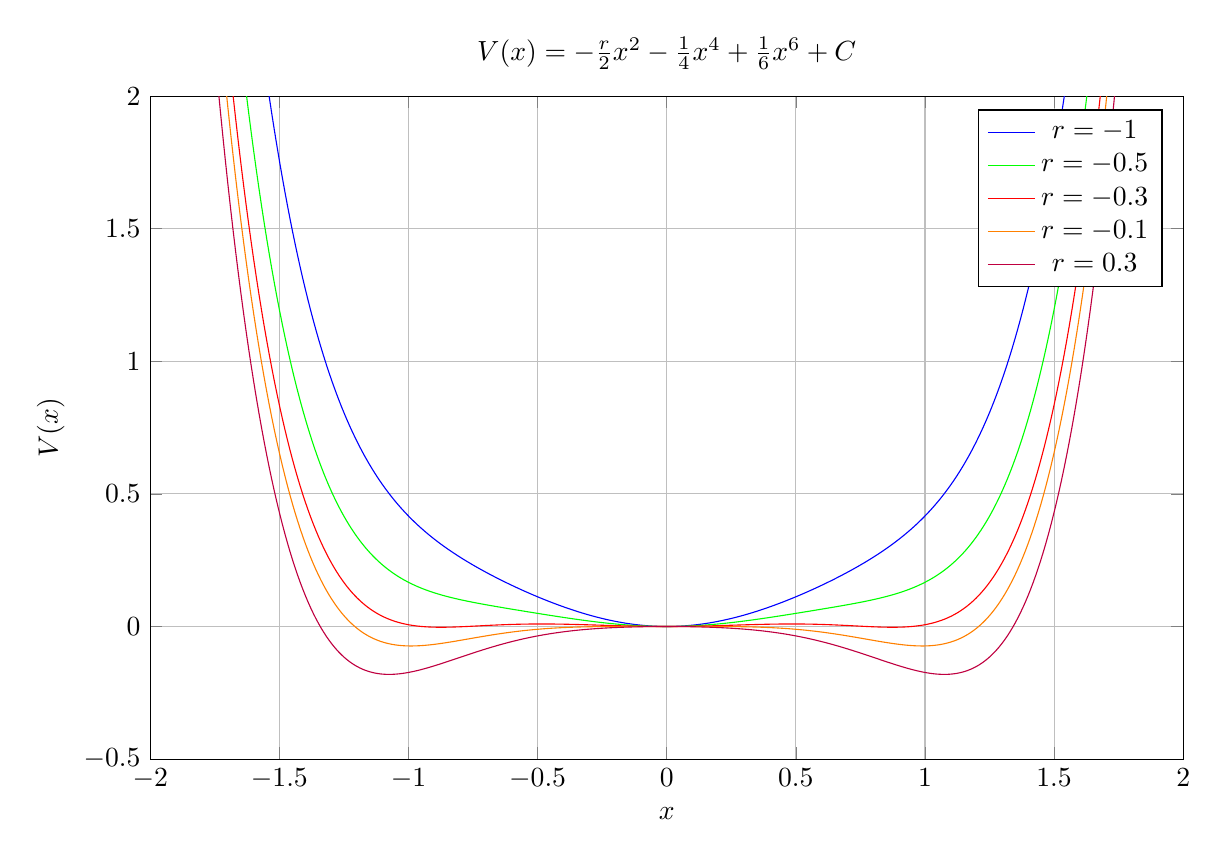
\begin{tikzpicture}
	\begin{axis}[
		title = {$V(x)= -\frac{r}{2}x^2-\frac{1}{4}x^4+\frac{1}{6}x^6+C$},
		xlabel = {$x$},
		ylabel = {$V(x)$},
		xmin = -2, xmax = 2,
		ymin = -0.5, ymax = 2,
		grid = major,
		width=14.7cm,
		height=10cm,
		]

		% when r=-1
		\addplot[blue, domain=-2:2, samples=400] {0.5*x^2-0.25*x^4+1/6*x^6};
		% when r=-0.5
		\addplot[green, domain=-2:2, samples=400] {0.25*x^2-0.25*x^4+1/6*x^6};
		% when r=-0.3
		\addplot[red, domain=-2:2, samples=400] {0.09*x^2-0.25*x^4+1/6*x^6};
		% when r=-0.1
		\addplot[orange, domain=-2:2, samples=400] {0.01*x^2-0.25*x^4+1/6*x^6};
		% when r=0.3
		\addplot[purple, domain=-2:2, samples=400] {-0.09*x^2-0.25*x^4+1/6*x^6};

		\legend{$r=-1$,$r=-0.5$,$r=-0.3$,$r=-0.1$,$r=0.3$}	
		\end{axis}
	\end{tikzpicture}

	\item Find the critical parameter values $r_c$ for the bifurcation points. We will use the $V'(x)=0$ to find the max/min values of $V(x)$. So we have:
	\[V'(x)=-rx^2-x^4+x^6=-x^2(r+x^2-x^4)=0.\]
	Then we have five critical points $x=0$ and
	\[x_1=\pm \sqrt{\frac{1-\sqrt{1+4r}}{\sqrt{2}}}, \quad x_2=\pm \sqrt{\frac{1+\sqrt{1+4r}}{\sqrt{2}}}.\]
	Now, let's analyze the critical points:
	
	Since the potential function is even, we only need to analyze the critical points $x=0$ and $x=\pm \sqrt{\frac{1+\sqrt{1+4r}}{\sqrt{2}}}$. Since $|x_2|>|x_1|$, we only need to analyze $x_2$, from the plot of $V(x)$, we can see that $x_2$ is a local minimum point if we want all the local minimum is $0$. Therefore, we will use $x_2$ to find the critical parameter values $r_c$ for the bifurcation points. So we have:
	\[V(x_2)=\frac{1}{2}\left(\frac{1+\sqrt{1+4r}}{\sqrt{2}}\right)^2-\frac{1}{4}\left(\frac{1+\sqrt{1+4r}}{\sqrt{2}}\right)^4+\frac{1}{6}\left(\frac{1+\sqrt{1+4r}}{\sqrt{2}}\right)^6=0.\]
	Then we have:
	\[ r_c = -\frac{3}{16}, \quad x_c = \frac{\sqrt{3}}{2}.\]

	So, the $V(x)$ with three local minimum values plot is below (When $C=0$ and $r=-3/16$):

	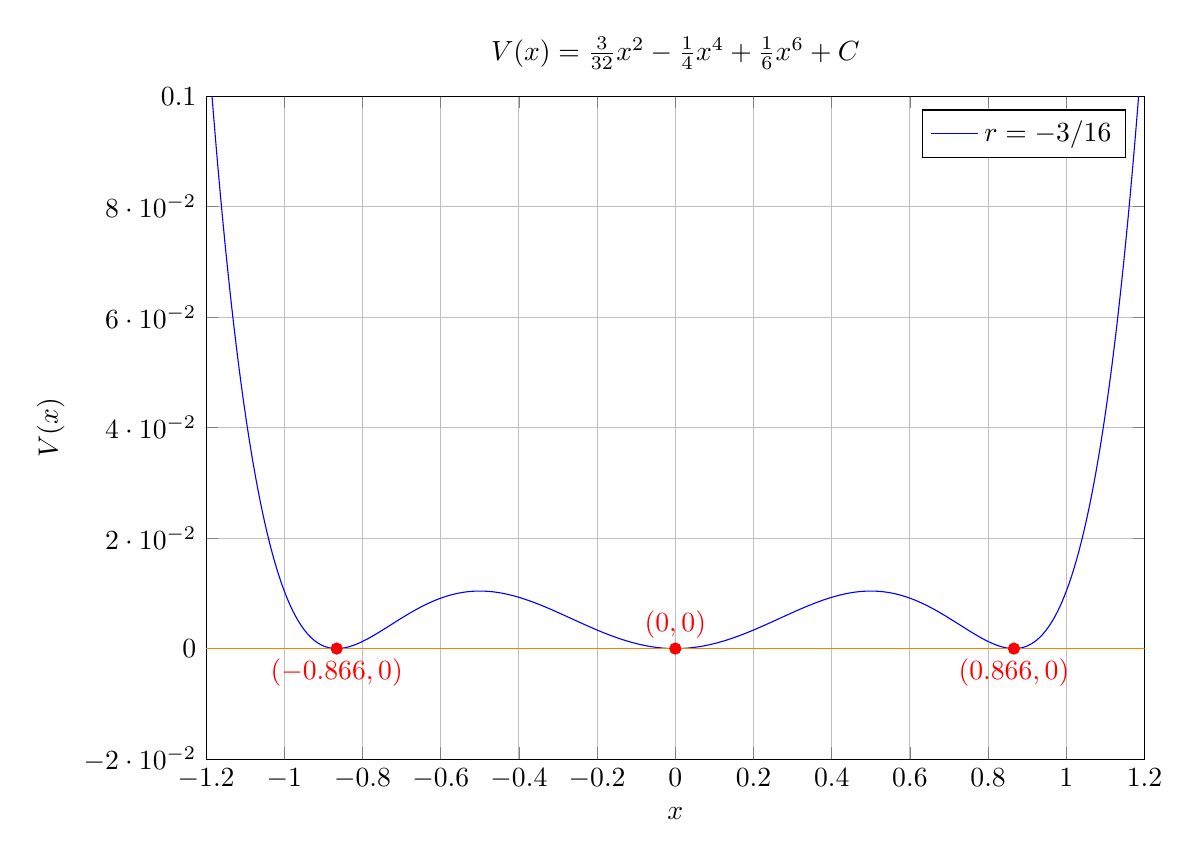
\begin{tikzpicture}
	\begin{axis}[
		title = {$V(x)= \frac{3}{32}x^2-\frac{1}{4}x^4+\frac{1}{6}x^6+C$},
		xlabel = {$x$},
		ylabel = {$V(x)$},
		xmin = -1.2, xmax = 1.2,	
		ymin = -0.02, ymax = 0.1,
		grid = major,
		width=13.5cm,
		height=10cm,
		]

		% when r=-3/16
		\addplot[blue, domain=-1.2:1.2, samples=400] {(3/32)*x^2-0.25*x^4+1/6*x^6};
		% add horizontal line x=0
		\addplot[orange, domain=-1.2:1.2, samples=100] {0};
		
		% add point at (0,0)
		\addplot[only marks, mark=*, mark size=2pt, color=red] coordinates {(0,0)} node[above]{$(0,0)$};
		% add point at (0.866,0)
		\addplot[only marks, mark=*, mark size=2pt, color=red] coordinates {(0.866,0)} node[below]{$(0.866,0)$};
		% add point at (-0.866,0)
		\addplot[only marks, mark=*, mark size=2pt, color=red] coordinates {(-0.866,0)} node[below]{$(-0.866,0)$};

		\legend{$r=-3/16$}
		\end{axis}
	\end{tikzpicture}
\end{enumerate}


\section*{Problem 5}
Consider the ODE $x'=rx-\sin x$.

\begin{enumerate}[(a)]
	\item For $r=0$, we have $x'=rx-\sin x=-\sin x$. The fixed points are $x=n\pi$ where $n \in \mathbb{Z}$. The fixed points are stable when $n$ is even and unstable when $n$ is odd. 

	\item For $r>1$, we can make a vector field plot below to see the behavior of the fixed points:

	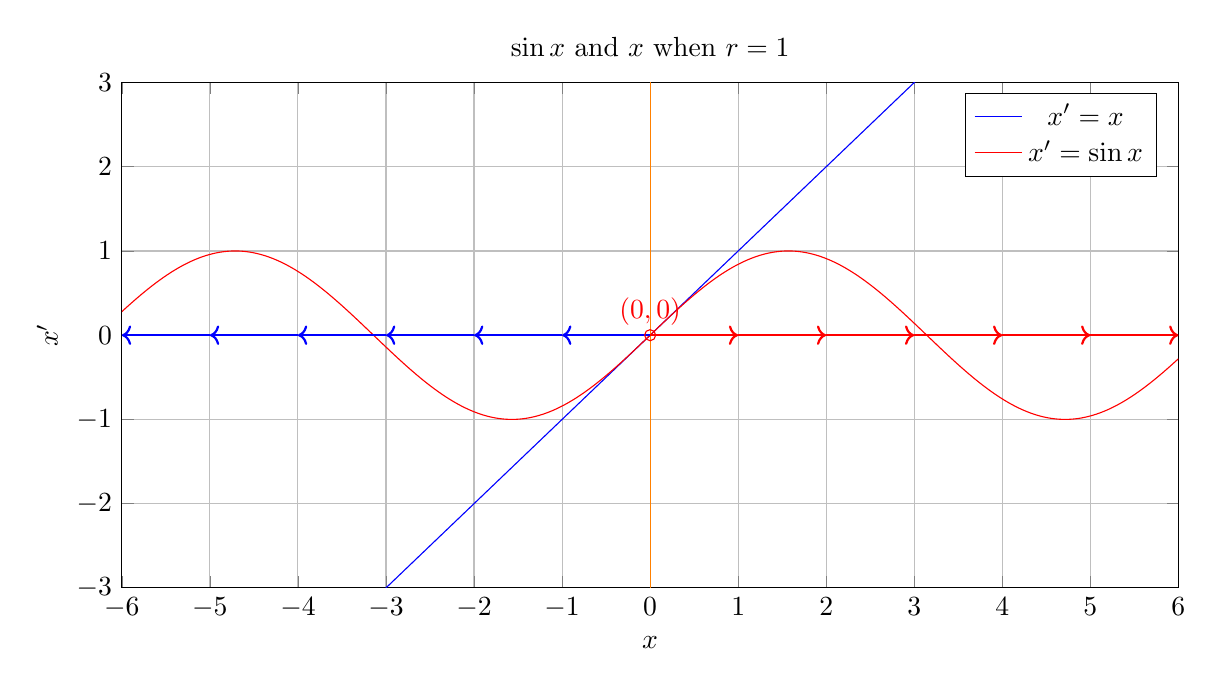
\begin{tikzpicture}
	\begin{axis}[
		title = {$\sin x$ and $x$ when $r=1$},
		xlabel = {$x$},
		ylabel = {$x'$},
		xmin = -6, xmax = 6,
		ymin = -3, ymax = 3,
		grid = major,
		width=15cm,
		height=8cm,
		]

		% when r=1 make y=x
		\addplot[blue, domain=-6:6, samples=400] {x};
		% plot sin(x) in red
		\addplot[red, domain=-6:6, samples=400] {sin(deg(x))};
		% add horizontal line x=0
		\addplot[orange, domain=-6:6, samples=100] {0};
		% add vertical line y=0
		\addplot[orange, domain=-6:6, samples=100] coordinates {(0,-3) (0,3)};
		
		% add hollow point at (0,0)
		\addplot[only marks, mark=o, mark size=2pt, color=red] coordinates {(0,0)} node[above]{$(0,0)$};

		% draw vector from (-5,0) to (-6,0) and change the arrow to thick
		\addplot[->, thick, color=blue] coordinates {(-5,0) (-6,0)};
		% draw vector from (-4,0) to (-5,0) and change the arrow to thick
		\addplot[->, thick, color=blue] coordinates {(-4,0) (-5,0)};
		% draw vector from (-3,0) to (-4,0) and change the arrow to thick
		\addplot[->, thick, color=blue] coordinates {(-3,0) (-4,0)};
		% draw vector from (-2,0) to (-3,0) and change the arrow to thick
		\addplot[->, thick, color=blue] coordinates {(-2,0) (-3,0)};
		% draw vector from (-1,0) to (-2,0) and change the arrow to thick
		\addplot[->, thick, color=blue] coordinates {(-1,0) (-2,0)};
		% draw vector from (0,0) to (-1,0) and change the arrow to thick
		\addplot[->, thick, color=blue] coordinates {(0,0) (-1,0)};

		% draw vector from (0,0) to (1,0) and change the arrow to thick
		\addplot[->, thick, color=red] coordinates {(0,0) (1,0)};
		% draw vector from (1,0) to (2,0) and change the arrow to thick
		\addplot[->, thick, color=red] coordinates {(1,0) (2,0)};
		% draw vector from (2,0) to (3,0) and change the arrow to thick
		\addplot[->, thick, color=red] coordinates {(2,0) (3,0)};
		% draw vector from (3,0) to (4,0) and change the arrow to thick
		\addplot[->, thick, color=red] coordinates {(3,0) (4,0)};
		% draw vector from (4,0) to (5,0) and change the arrow to thick
		\addplot[->, thick, color=red] coordinates {(4,0) (5,0)};
		% draw vector from (5,0) to (6,0) and change the arrow to thick
		\addplot[->, thick, color=red] coordinates {(5,0) (6,0)};


		\legend{$x'=x$,$x'=\sin x$}
		\end{axis}
	\end{tikzpicture}
	
	Since $x> \sin x$ for $x>0$ and $x< \sin x$ for $x<0$ and $kx>x$ for all $k \in \mathbb{Z_{+}}$, we can see that the fixed point $x=0$ is unstable. 
	
	\item As we did before, we found that there is one fixed point $x=0$ when $r \in [1, \infty)$. A subcritical pitchfork bifurcation occurs at $r = 1$ as two fixed points are created. As $r$ keep decreasing from $1$ to $0$ the $rx$ will intersect with $\sin x$ more even fixed poins each time which is creating many saddle-node bifurcations.

	\item The increasing from $-\infty$ to $0$ is similar to the decreasing from $-\infty$ to $0$. The fixed point $x=0$ is stable before around $r=-0.22$ and then will more even fixed points each time which is creating many saddle-node bifurcations.

	\item Based on the analysis above, we can make the bifurcation diagram of $x$ vs. $r$ below:
	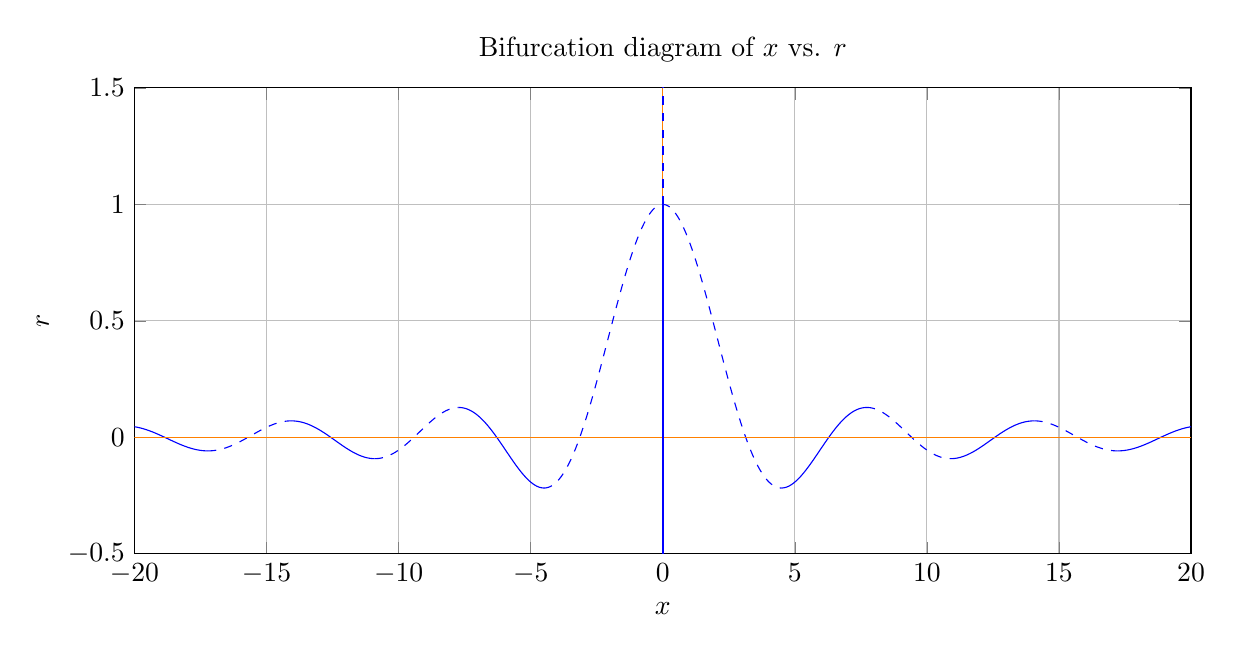
\begin{tikzpicture}
	\begin{axis}[
		title = {Bifurcation diagram of $x$ vs. $r$},
		xlabel = {$x$},
		ylabel = {$r$},
		xmin = -20, xmax = 20,
		ymin = -0.5, ymax = 1.5,
		grid = major,
		width=15cm,
		height=7.5cm,
		]

		% sin(x)/x where x \in [-4.493,4.493] with dash line
		\addplot[blue, domain=-4.493:4.493, samples=200, dashed] {sin(deg(x))/x};
		% sin(x)/x where x \in [-7.725, -4.493] 
		\addplot[blue, domain=-7.725:-4.493, samples=200] {sin(deg(x))/x};
		% sin(x)/x where x \in [-10.904, -7.725] with dash line
		\addplot[blue, domain=-10.904:-7.725, samples=200, dashed] {sin(deg(x))/x};
		% sin(x)/x where x \in [-14.066, -10.904]
		\addplot[blue, domain=-14.066:-10.904, samples=200] {sin(deg(x))/x};
		% sin(x)/x where x \in [-17.220, -14.066] with dash line
		\addplot[blue, domain=-17.220:-14.066, samples=200, dashed] {sin(deg(x))/x};
		% sin(x)/x where x \in [-20, -17.220]
		\addplot[blue, domain=-20:-17.220, samples=200] {sin(deg(x))/x};
		
		% sin(x)/x where x \in [4.493, 7.725]
		\addplot[blue, domain=4.493:7.725, samples=200] {sin(deg(x))/x};
		% sin(x)/x where x \in [7.725, 10.904] with dash line
		\addplot[blue, domain=7.725:10.904, samples=200, dashed] {sin(deg(x))/x};
		% sin(x)/x where x \in [10.904, 14.066]
		\addplot[blue, domain=10.904:14.066, samples=200] {sin(deg(x))/x};
		% sin(x)/x where x \in [14.066, 17.220] with dash line
		\addplot[blue, domain=14.066:17.220, samples=200, dashed] {sin(deg(x))/x};
		% sin(x)/x where x \in [17.220, 20]
		\addplot[blue, domain=17.220:20, samples=200] {sin(deg(x))/x};

		% add horizontal line x=0
		\addplot[orange, domain=-20:20, samples=100] {0};
		% add vertical line y=0
		\addplot[orange, domain=-20:20, samples=100] coordinates {(0,-0.5) (0,1.5)};
		% add vertical line y=0 from x=1 to x=2 dash line
		\addplot[blue, domain=-20:20, samples=100, dashed, thick] coordinates {(0,1) (0,2)};
		% add vertical line y=0 from x=1 to x=-0.5
		\addplot[blue, domain=-20:20, samples=100, thick] coordinates {(0,1) (0,-0.5)};
		
		\end{axis}
	\end{tikzpicture}

\end{enumerate}


















\end{document}

